\documentclass{scrartcl}

%\usepackage{etex}
\usepackage[left=3cm,right=2.0cm,top=1.25cm,bottom=1.75cm,includehead,includefoot]
{geometry}
\usepackage{marginnote}
\reversemarginpar
%Math
\usepackage{amsfonts,amsmath,amssymb,amsthm, amstext}
%Language, encoding, ...
\usepackage[utf8]{inputenc}
\usepackage[T1]{fontenc}
\usepackage[english]{babel}
\usepackage{t1enc, lmodern, textcomp}
%Pictures
\usepackage{graphicx, color}
%\usepackage{latexsym}
%\usepackage{keyval}
%\usepackage{ifthen}
%\usepackage{moreverb}
\usepackage[shell]{gnuplottex}
%Colors
\usepackage[usenames,dvipsnames]{xcolor}
\definecolor{darkblue}{rgb}{0.0, 0.2, 0.6}
\renewcommand*{\marginfont}{\bf\color{darkblue}}
%Nice a/b fractions
\usepackage{xfrac}
%Make it possible to write (fat) upright greek letters
\usepackage{upgreek}

%For indices
\newcommand{\ix}[1]{_{\mathrm{#1}}}
\newcommand{\Ix}[1]{^{\mathrm{#1}}}

%Directly include svg images
%%%%%%%%%%%%%%%%%%%%%%%%%%%%%%%%%%%%%%%%%%%%%%%%%%
\newcommand{\executeiffilenewer}[3]{%
    \ifnum\pdfstrcmp{\pdffilemoddate{#1}}%
    {\pdffilemoddate{#2}}>0%
    {\immediate\write18{#3}}\fi%
}
\newcommand{\includesvg}[1]{%
    \executeiffilenewer{#1.svg}{#1.pdf}%
    {inkscape -z -D --file=#1.svg %
    --export-pdf=#1.pdf --export-latex}%
    \input{#1.pdf_tex}%
}
%%%%%%%%%%%%%%%%%%%%%%%%%%%%%%%%%%%%%%%%%%%%%%%%%%

%Make captions look okay
\usepackage[font=small,format=plain,labelfont=bf,up,up]{caption}

%Hyperlinks
\usepackage{hyperref}
\hypersetup{
            pdflang=en-EN,
            unicode=true,
            pdfauthor={Thomas Staudt, Erik Schultheis},
}

%Differential d's
\newcommand{\dif}{\mathrm{d}}
\newcommand{\tdif}[2]{\ensuremath{\frac{\dif#1}{\dif#2}}}
\newcommand{\pdif}[2]{\ensuremath{\frac{\partial#1}{\partial#2}}}
\newcommand{\ppdif}[2]{\ensuremath{\frac{\partial^{2}#1}{\partial#2^{2}}}}
%Degree
\newcommand{\degr}{^\circ}

\renewcommand{\refname} {Literature}
\renewcommand{\figurename}{\bf Figure}
\newcommand{\fs}[1]{\footnotesize #1}
%double slash
\newcommand{\git}{\mathbin{
  \mathchoice{\textbackslash\mkern-6mu\textbackslash}% \displaystyle
    {\textbackslash\mkern-6mu\textbackslash}% \textstyle
    {\textbackslash\mkern-5mu\textbackslash}% \scriptstyle
    {\textbackslash\mkern-5mu\textbackslash}}}% \scriptscriptstyle


%Bibliography
\usepackage[babel]{csquotes}
\usepackage[backend=bibtex8]{biblatex}


\newcommand*{\defeq}{\mathrel{\vcenter{\baselineskip0.5ex \lineskiplimit0pt
                     \hbox{\scriptsize.}\hbox{\scriptsize.}}}%
                     =}



%\bibliography{sources}


\begin{document}

\begin{titlepage}\centering
\textsc{\Large Institute For Nonlinear Dynamics \\[1.5ex] Universität Göttingen}

\vspace*{2cm}
{\huge A Practical Course On Network Science}
\vspace*{2cm}

\rule{\textwidth}{1pt}\\[0.5cm]
{\bfseries \huge Block A: \\[0.5cm] \huge \bfseries Random Networks\\[0.5cm]}
\rule{\textwidth}{1pt}

\vspace*{4cm}

\begin{Large}\begin{tabular}{rl}
        \textbf{Participants:}  & Erik Schultheis                                \\    
                   & \textit{erik.schultheis@stud.uni-goettingen.de}\\[0.5cm]
                   & Thomas Staudt                                  \\
                   & \textit{thomas.staudt@stud.uni-goettingen.de}  \\[1.0cm]

       \textbf{Tutors:}        & Dr. Nora Molkenthin, Benjamin Schäfer, Malte Schröder  \\[1.0cm]
       \textbf{Deadline:}      & 21.05.2015
\end{tabular}\end{Large}

\vspace*{1.5cm}

%\begin{Large}
%\fbox{
  %\begin{minipage}[t][2.5cm][t]{6cm} 
      %Attestation:
  %\end{minipage}
%}
%\end{Large} 

\end{titlepage}

\tableofcontents
\clearpage

\section{Random Networks}
\subsection{Task 1}
\subsection{Task 2}
\subsection{Task 3}
\subsection{Task 4}
\subsection{Task 5}

\section{Scale-Free Networks and Robustness}
\subsection{Generating and Visualizing Barab\'asi-Albert}

\begin{figure}
    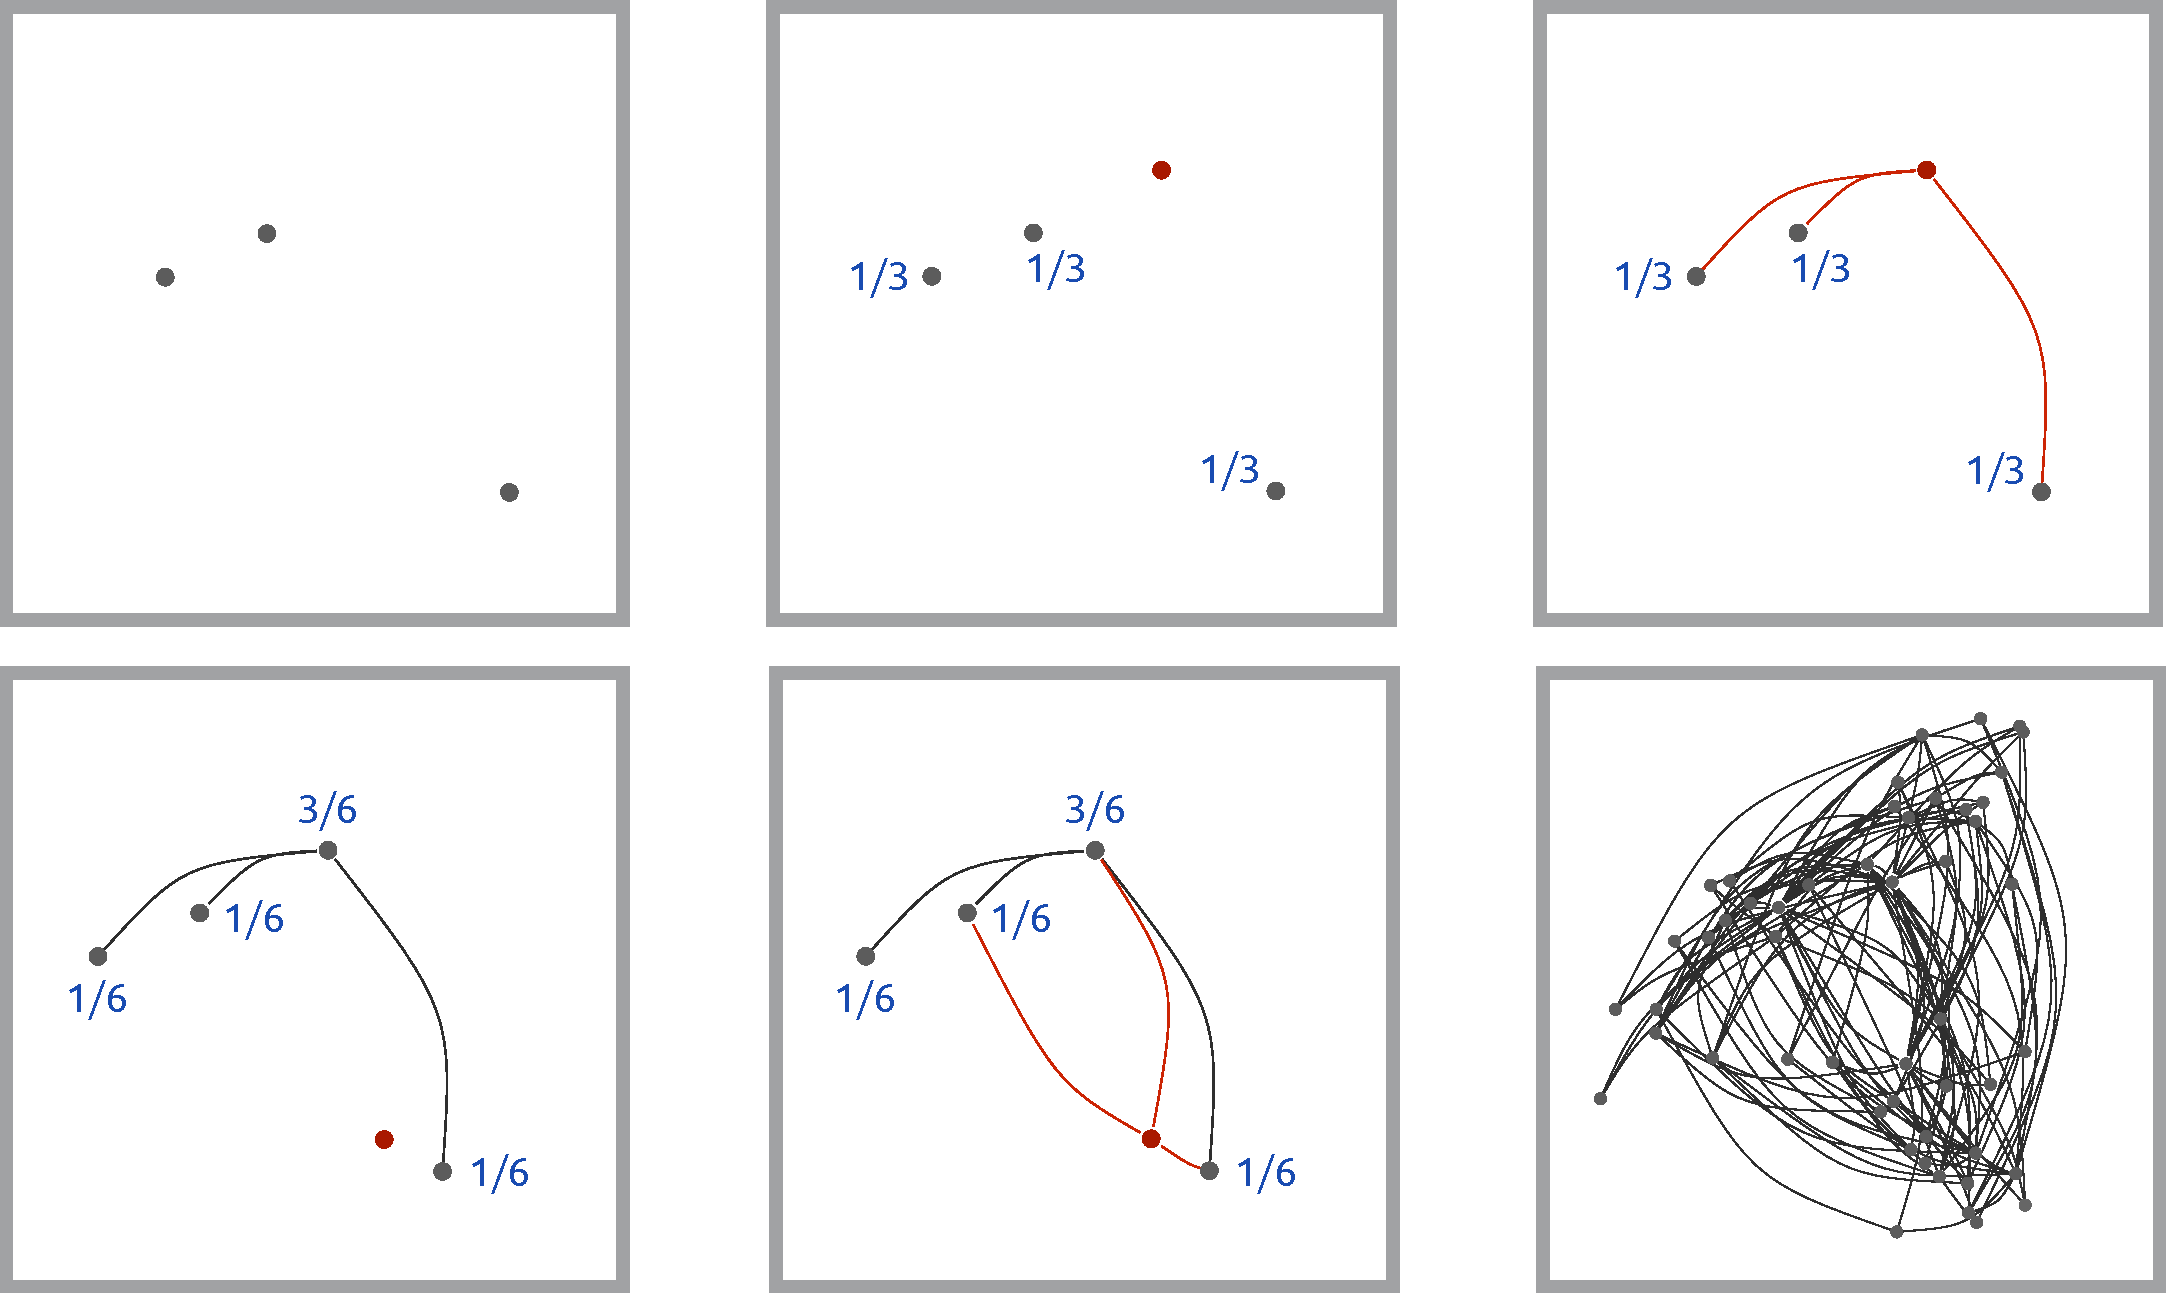
\includegraphics[width=\textwidth]{pictures/21_begin.pdf}
    \caption{The first steps of the Barab\'asi-Albert algorithm with $m
    = m_0 = 3$. From left to right and from top to bottom single nodes are
    first added before edges are chosen according to the preferential
    attachment probabilities printed in blue. The last picture shows the network
    after 47 nodes have been added.}
    \label{fig:21_begin}
\end{figure}

\begin{figure}
    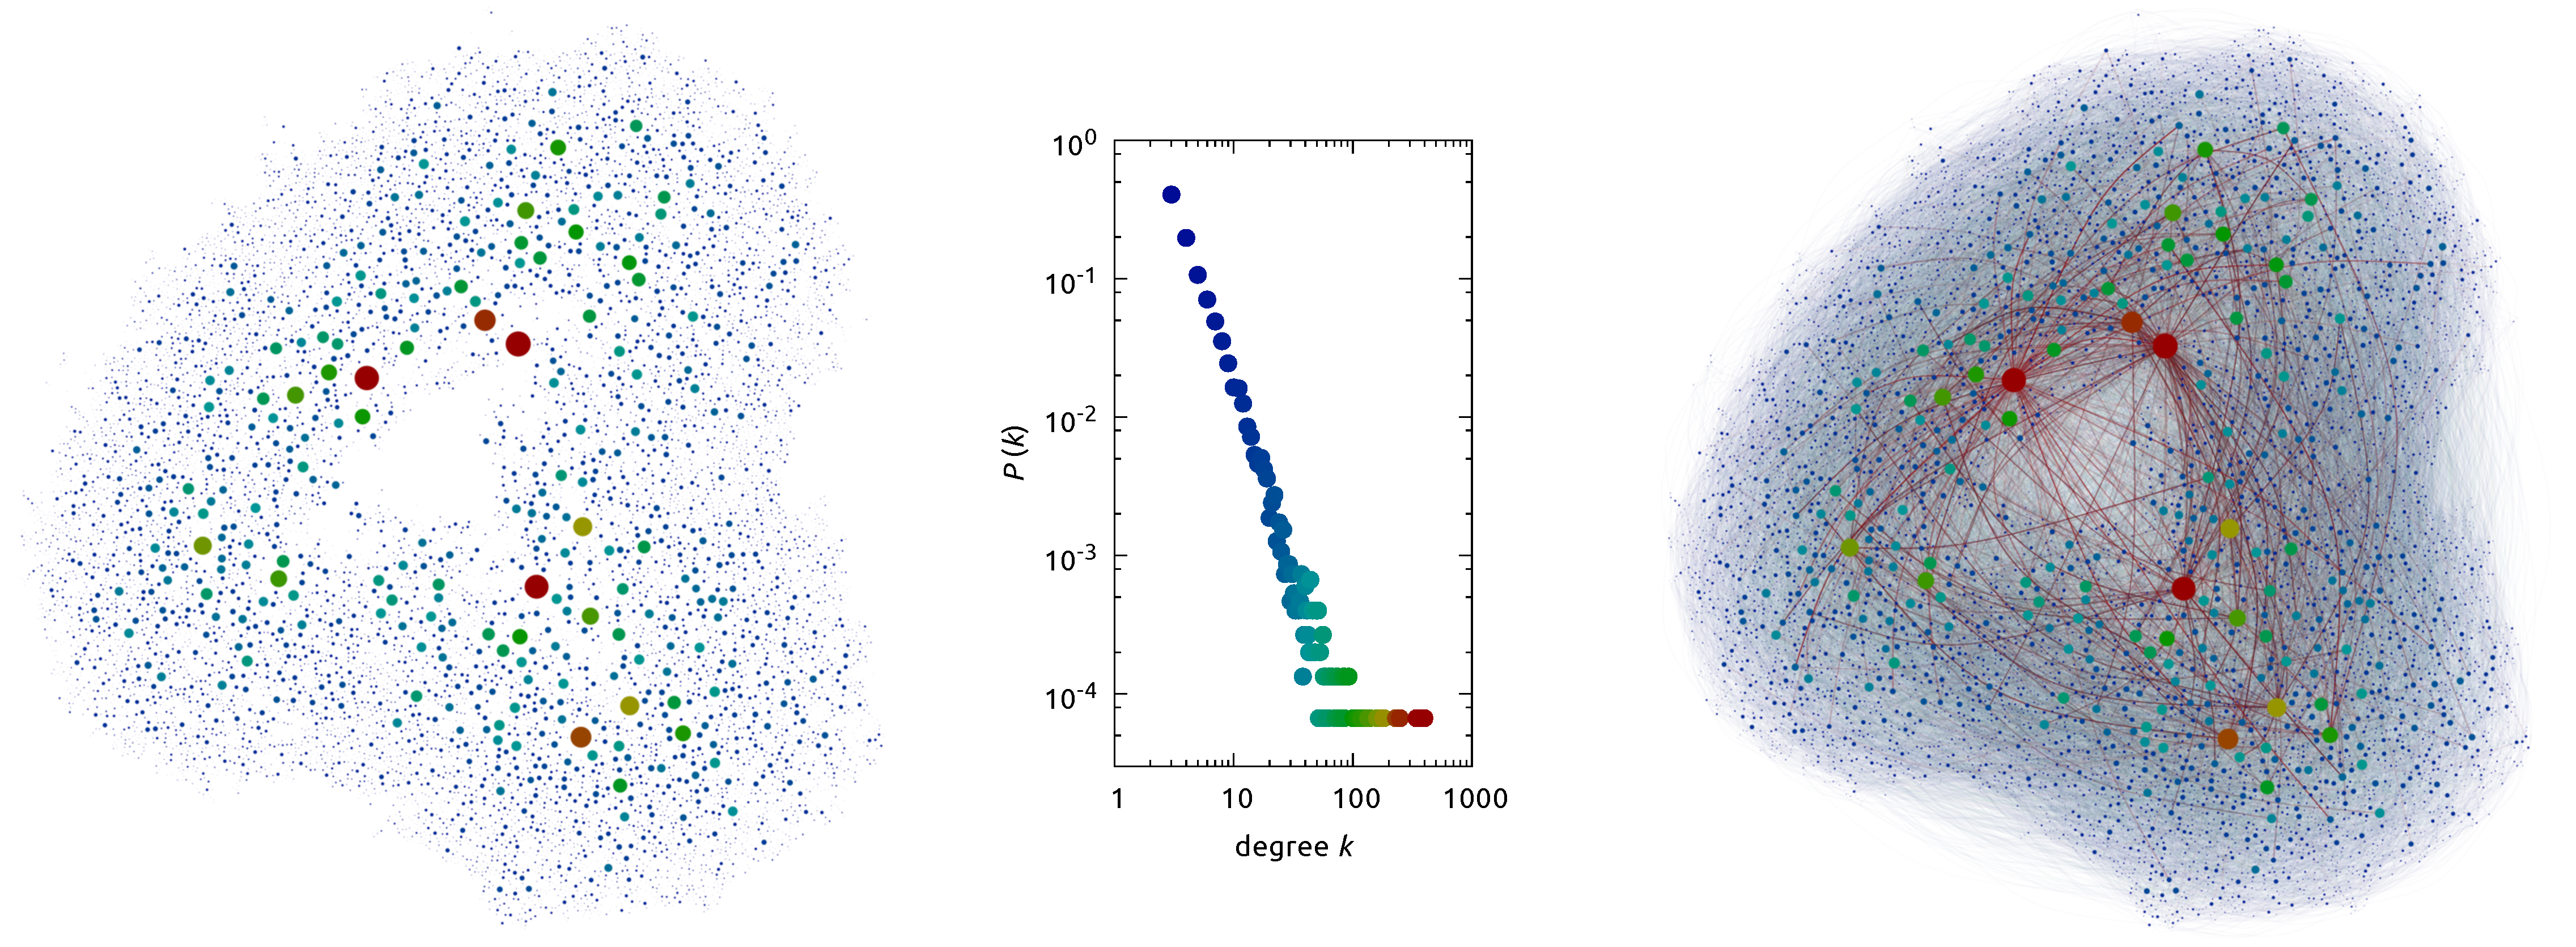
\includegraphics[width=\textwidth]{pictures/21_end.pdf}
    \caption{The same network as in figure \ref{fig:21_begin} after 15000
    nodes have been added (left: without drawing the edges, and right: with
    drawing the edges). The color and the size of the nodes printed in the left
    and right picture describe the degree of the respective node. The
    picture in the middle shows the degree distribution (with the same color
    keys as in the node coloring).}
    \label{fig:21_end}
\end{figure}

\subsection{The Degree Distribution of Barab\'asi-Albert Algorithm}
\begin{figure}
    \gnuplotloadfile[terminal=epslatex, terminaloptions={color size 6,3}]{pictures/22_plot.gp}
    \caption{Degree distribution for a simulation with $N=500000$ nodes
    in total, using different values for $m=m_0$. The line has a slope of
    $-3$.}
    \label{fig:22_plot}
\end{figure}
\begin{figure}
    \gnuplotloadfile[terminal=epslatex, terminaloptions={color size 6,3}]{pictures/22_logplot.gp}
    \caption{The same degree distribution as in figure \ref{fig:22_plot}
    using logarithmic binning so that the the points plotted are the average
    values over equidistant bins on the logarithmic axis (i.e. the bin width
    increases exponentially).}
    \label{fig:22_logplot}
\end{figure}

\subsection{Task 3}
\subsection{Task 4}
\subsection{Task 5}

\end{document}
